% Source: graduate-coursework/Research/Intro_to_Agents/handouts/Part8_Advanced_Topics.tex

\documentclass[border=4pt]{standalone}
\usepackage[T1]{fontenc}
\usepackage{graphicx}
\usepackage{lmodern}
\usepackage{tikz}
\usepackage{xcolor}
\usetikzlibrary{shapes.geometric, arrows.meta, positioning, calc, fit, backgrounds, matrix, decorations.pathreplacing}

\definecolor{UofSCGarnet}{HTML}{73000a}
\definecolor{UofSCBlack}{HTML}{000000}
\definecolor{UofSCWhite}{HTML}{ffffff}
\definecolor{UofSCRose}{HTML}{CC2E40}
\definecolor{UofSCAtlantic}{HTML}{466A9F}
\definecolor{UofSCCongaree}{HTML}{1F414D}
\definecolor{UofSCHorseshoe}{HTML}{65780B}
\definecolor{UofSCGrass}{HTML}{CED318}
\definecolor{UofSCHoneycomb}{HTML}{A49137}
\definecolor{UofSC90Black}{HTML}{363636}
\definecolor{UofSC70Black}{HTML}{5C5C5C}
\definecolor{UofSC50Black}{HTML}{A2A2A2}
\definecolor{UofSCWarmGrey}{HTML}{676156}
\definecolor{UofSCSandstorm}{HTML}{FFF2E3}
\definecolor{UofSCDarkGarnet}{HTML}{570008}
\definecolor{UofSCAzalea}{HTML}{844247}

\tikzset{
    % Sharp corners for all nodes
    every node/.style={font=\small},
    % Process box style
    process/.style={
        rectangle,
        draw=UofSCBlack,
        fill=UofSCWhite,
        minimum width=2.5cm,
        minimum height=0.8cm,
        align=center,
        font=\footnotesize
    },
    % Decision box style
    decision/.style={
        diamond,
        draw=UofSCBlack,
        fill=UofSCSandstorm,
        minimum width=2cm,
        minimum height=1cm,
        align=center,
        font=\footnotesize,
        aspect=2
    },
    % Start/End style
    startstop/.style={
        rectangle,
        draw=UofSCGarnet,
        fill=UofSCGarnet,
        text=UofSCWhite,
        minimum width=2cm,
        minimum height=0.7cm,
        align=center,
        font=\footnotesize\bfseries
    },
    % Arrow style
    arrow/.style={
        ->,
        >=Stealth,
        thick,
        color=UofSCBlack
    },
    % Failure node
    failure/.style={
        rectangle,
        draw=UofSCRose,
        fill=UofSCRose!20,
        minimum width=2cm,
        minimum height=0.7cm,
        align=center,
        font=\footnotesize
    },
    % Success node
    success/.style={
        rectangle,
        draw=UofSCHorseshoe,
        fill=UofSCHorseshoe!20,
        minimum width=2cm,
        minimum height=0.7cm,
        align=center,
        font=\footnotesize
    },
    % Highlight box
    highlight/.style={
        rectangle,
        draw=UofSCGarnet,
        fill=UofSCGarnet!10,
        line width=1.5pt,
        minimum width=2.5cm,
        minimum height=0.8cm,
        align=center,
        font=\footnotesize
    },
    % Security threat style
    threat/.style={
        rectangle,
        draw=UofSCRose,
        fill=UofSCRose!15,
        minimum width=2.2cm,
        minimum height=0.7cm,
        align=center,
        font=\footnotesize
    },
    % Agent node
    agent/.style={
        rectangle,
        draw=UofSCAtlantic,
        fill=UofSCAtlantic!15,
        minimum width=2.2cm,
        minimum height=0.8cm,
        align=center,
        font=\footnotesize
    },
    % Human node
    human/.style={
        rectangle,
        draw=UofSCCongaree,
        fill=UofSCCongaree!15,
        minimum width=2.2cm,
        minimum height=0.8cm,
        align=center,
        font=\footnotesize
    },
    % Cost node
    cost/.style={
        rectangle,
        draw=UofSCHoneycomb,
        fill=UofSCHoneycomb!20,
        minimum width=2cm,
        minimum height=0.7cm,
        align=center,
        font=\footnotesize
    },
    % Test node
    test/.style={
        rectangle,
        draw=UofSCAtlantic,
        fill=UofSCAtlantic!10,
        minimum width=2cm,
        minimum height=0.7cm,
        align=center,
        font=\footnotesize
    },
    % Pipeline stage
    pipeline/.style={
        rectangle,
        draw=UofSCCongaree,
        fill=UofSCCongaree!10,
        minimum width=2.5cm,
        minimum height=0.8cm,
        align=center,
        font=\footnotesize
    },
    % Timeline event
    timeline/.style={
        rectangle,
        draw=UofSCGarnet,
        fill=UofSCWhite,
        minimum width=1.8cm,
        minimum height=0.6cm,
        align=center,
        font=\tiny
    }
}

\begin{document}
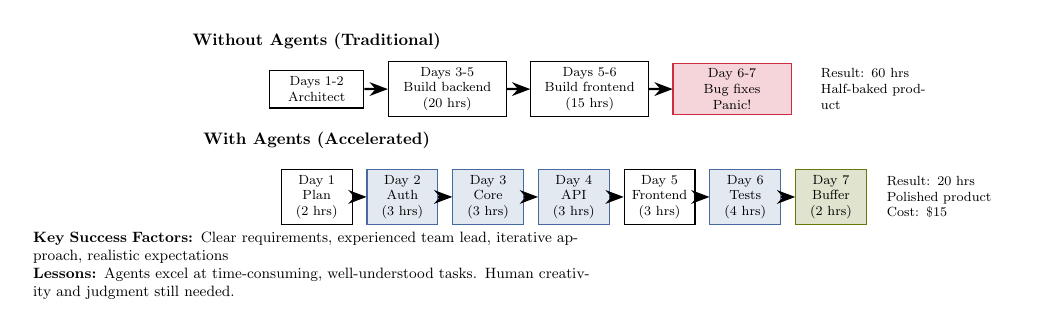
\begin{tikzpicture}[node distance=0.3cm and 1cm, scale=0.6, transform shape]
        % Timeline comparison
        \node (title1) [font=\bfseries] {Without Agents (Traditional)};
        \node (d1) [process, below=0.3cm of title1, minimum width=2cm] {Days 1-2\\Architect};
        \node (d2) [process, right=0.5cm of d1, minimum width=2.5cm] {Days 3-5\\Build backend\\(20 hrs)};
        \node (d3) [process, right=0.5cm of d2, minimum width=2.5cm] {Days 5-6\\Build frontend\\(15 hrs)};
        \node (d4) [failure, right=0.5cm of d3, minimum width=2.5cm] {Day 6-7\\Bug fixes\\Panic!};

        \draw [arrow] (d1) -- (d2);
        \draw [arrow] (d2) -- (d3);
        \draw [arrow] (d3) -- (d4);

        \node [right=0.5cm of d4, font=\footnotesize, text width=2.5cm] {Result: 60 hrs\\Half-baked product};

        % With agents
        \node (title2) [font=\bfseries, below=1.5cm of title1] {With Agents (Accelerated)};
        \node (a1) [process, below=0.3cm of title2, minimum width=1.5cm] {Day 1\\Plan\\(2 hrs)};
        \node (a2) [agent, right=0.3cm of a1, minimum width=1.5cm] {Day 2\\Auth\\(3 hrs)};
        \node (a3) [agent, right=0.3cm of a2, minimum width=1.5cm] {Day 3\\Core\\(3 hrs)};
        \node (a4) [agent, right=0.3cm of a3, minimum width=1.5cm] {Day 4\\API\\(3 hrs)};
        \node (a5) [process, right=0.3cm of a4, minimum width=1.5cm] {Day 5\\Frontend\\(3 hrs)};
        \node (a6) [agent, right=0.3cm of a5, minimum width=1.5cm] {Day 6\\Tests\\(4 hrs)};
        \node (a7) [success, right=0.3cm of a6, minimum width=1.5cm] {Day 7\\Buffer\\(2 hrs)};

        \draw [arrow] (a1) -- (a2);
        \draw [arrow] (a2) -- (a3);
        \draw [arrow] (a3) -- (a4);
        \draw [arrow] (a4) -- (a5);
        \draw [arrow] (a5) -- (a6);
        \draw [arrow] (a6) -- (a7);

        \node [right=0.3cm of a7, font=\footnotesize, text width=2.5cm] {Result: 20 hrs\\Polished product\\Cost: \$15};

        % Key factors
        \node [below=1.5cm of title2, text width=12cm, font=\small] {
            \textbf{Key Success Factors:} Clear requirements, experienced team lead, iterative approach, realistic expectations\\
            \textbf{Lessons:} Agents excel at time-consuming, well-understood tasks. Human creativity and judgment still needed.
        };
    \end{tikzpicture}
\end{document}
